\section{Discussion}
\label{sec:discussions}

We have carried out a first comprehensive comparison of the EHT 2017 \sgra data to a state-of-the-art library of numerical models.  None of the models survive the full gauntlet of 11 heterogeneous observational constraints.  In our standard model set, however, a cluster of strongly magnetized (MAD) models at intermediate inclination, positive spin, and large ($\Rh \ge 40$) ion-electron temperature ratios survives 10/11 constraints.  The standout constraint is the light curve variability, $\mi{3}$.


%==============================================================================
\subsection{MAD, SANE, and Self-Consistent Wind Feeding}

\note{Angelo to provide first draft}

There are clear differences between MAD and SANE models in VLBI data, as well as in the non-VLBI data.

Assessment of Ressler model.  Viable!

%==============================================================================
\subsection{Electron Distribution Function}

\note{Koushik to provide first draft}

Strong constraint on abundance of cold electrons from bremss.  A high density of cold electrons - which would be invisible in synchrotron - are ruled out.  This is in part because at $\Theta_e \equiv k T_e/(m_e c^2) \lesssim 1$, $j_\nu \propto \Theta_e^{-1/2}$ (emission in the x-ray band increases as temperature decreases).  In contrast, for $\Theta_e \gtrsim 1$ electron-electron bremsstrahlung becomes important and $j_\nu \propto \Theta_e^{+1/2}$.

Strong constraint on abundance of hot electrons from NIR.  In particular for

Strong constraint on $T_i/T_e$: models with ion temperature equal to electron temperature fail on several counts.

%==============================================================================
\subsection{Inclination}

\note{Michi to provide first draft}
\note{Strong constraints on inclination from m-ring fitting.}
\ckc{ck's first pass}

When the accretion flow around a black hole has enough angular momentum, the corresponding black hole image is sensitive to its inclination---in an edge-on case, the image is more asymmetric, with one side lighted up because of Doppler boosting; for a face-on case, the image is a more symmetric ring.
\gw{I agree with the preceding, but I'm worried that this may be misleading with respect to how the geometry of the spacetime influences the image. For example, even if the flow angular momentum is zero, if bhspin > 0, then the corresponding image is *still* sensitive to inclination.}
\ckc{Good point.  Feel free to edit.}
However, this dependency is weak in a low angular moment accretion flow, or when frame dragging cancels out the Doppler effect. These situations include the MAD state, where the accretion flow is magnetically supported, and retrograde accretion flows \citep{2021arXiv210503424M}.

The above conditional dependency of the asymmetry of the ring and
inclination makes it non-trivial to measure inclination from the
observation.
In addition, it is important to note that the asymmetry described
above does not directly corresponds to the m-ring asymmetry.
Consider a situation that the Doppler boosting is so extreme that only
the bright side of the photon ring is visible, while the dim side is
hidden under the noise.
In such a situation, the m-ring (or the gm-ring in \citetalias{PaperIV})
may misidentify the boosted side as the full image, and return a low
asymmetry, small image size, and wide image width.
This is the reason that it is difficult to directly link one m-ring
measurement to the inclination.
Nevertheless, given that the EHT observation is surprisingly
symmetric, the m-ring asymmetry measurement is not constraining.
In stead, the m-ring size disfavors the face-on images.

%==============================================================================
\subsection{Position Angle}

\note{Virtually no constraint on position angle [check m-ring fits]}

According to the data, the image of \sgra is surprisingly symmetric.
The position angle measurement is dominated by noise.
Our visibility domain constraining is therefore not constrianing on
the position angle.

%==============================================================================
\subsection{Black Hole Spin}

\note{Still quite weak constraints on black hole spin.}

Given that the size and the shape of the black hole shadow is
insensitive to its spin, the black hole spin remains one of the most
difficult black hole parameters to constraint.

However, as we discussed earlier, the asymmetry of the image does
depend on the black hole spin, assuming that there is significant
angular momentum in the accretion flow, In this sense, the
astrophysics can help us narrow down the spin.
Specifically, the m-ring diameter disfavors low spin models.
However, with the current u uncertainties in, e.g., the eDF, we are
not be able to report an acutal spin measurement.

%==============================================================================
\subsection{Accretion Rate and Outflow Power}

\monika{this section has been revised, please check and revise further}

%figures go first to align them with text better
% these plots should be shown together because they share rhigh label, so I merged them
\begin{figure*}
\centering
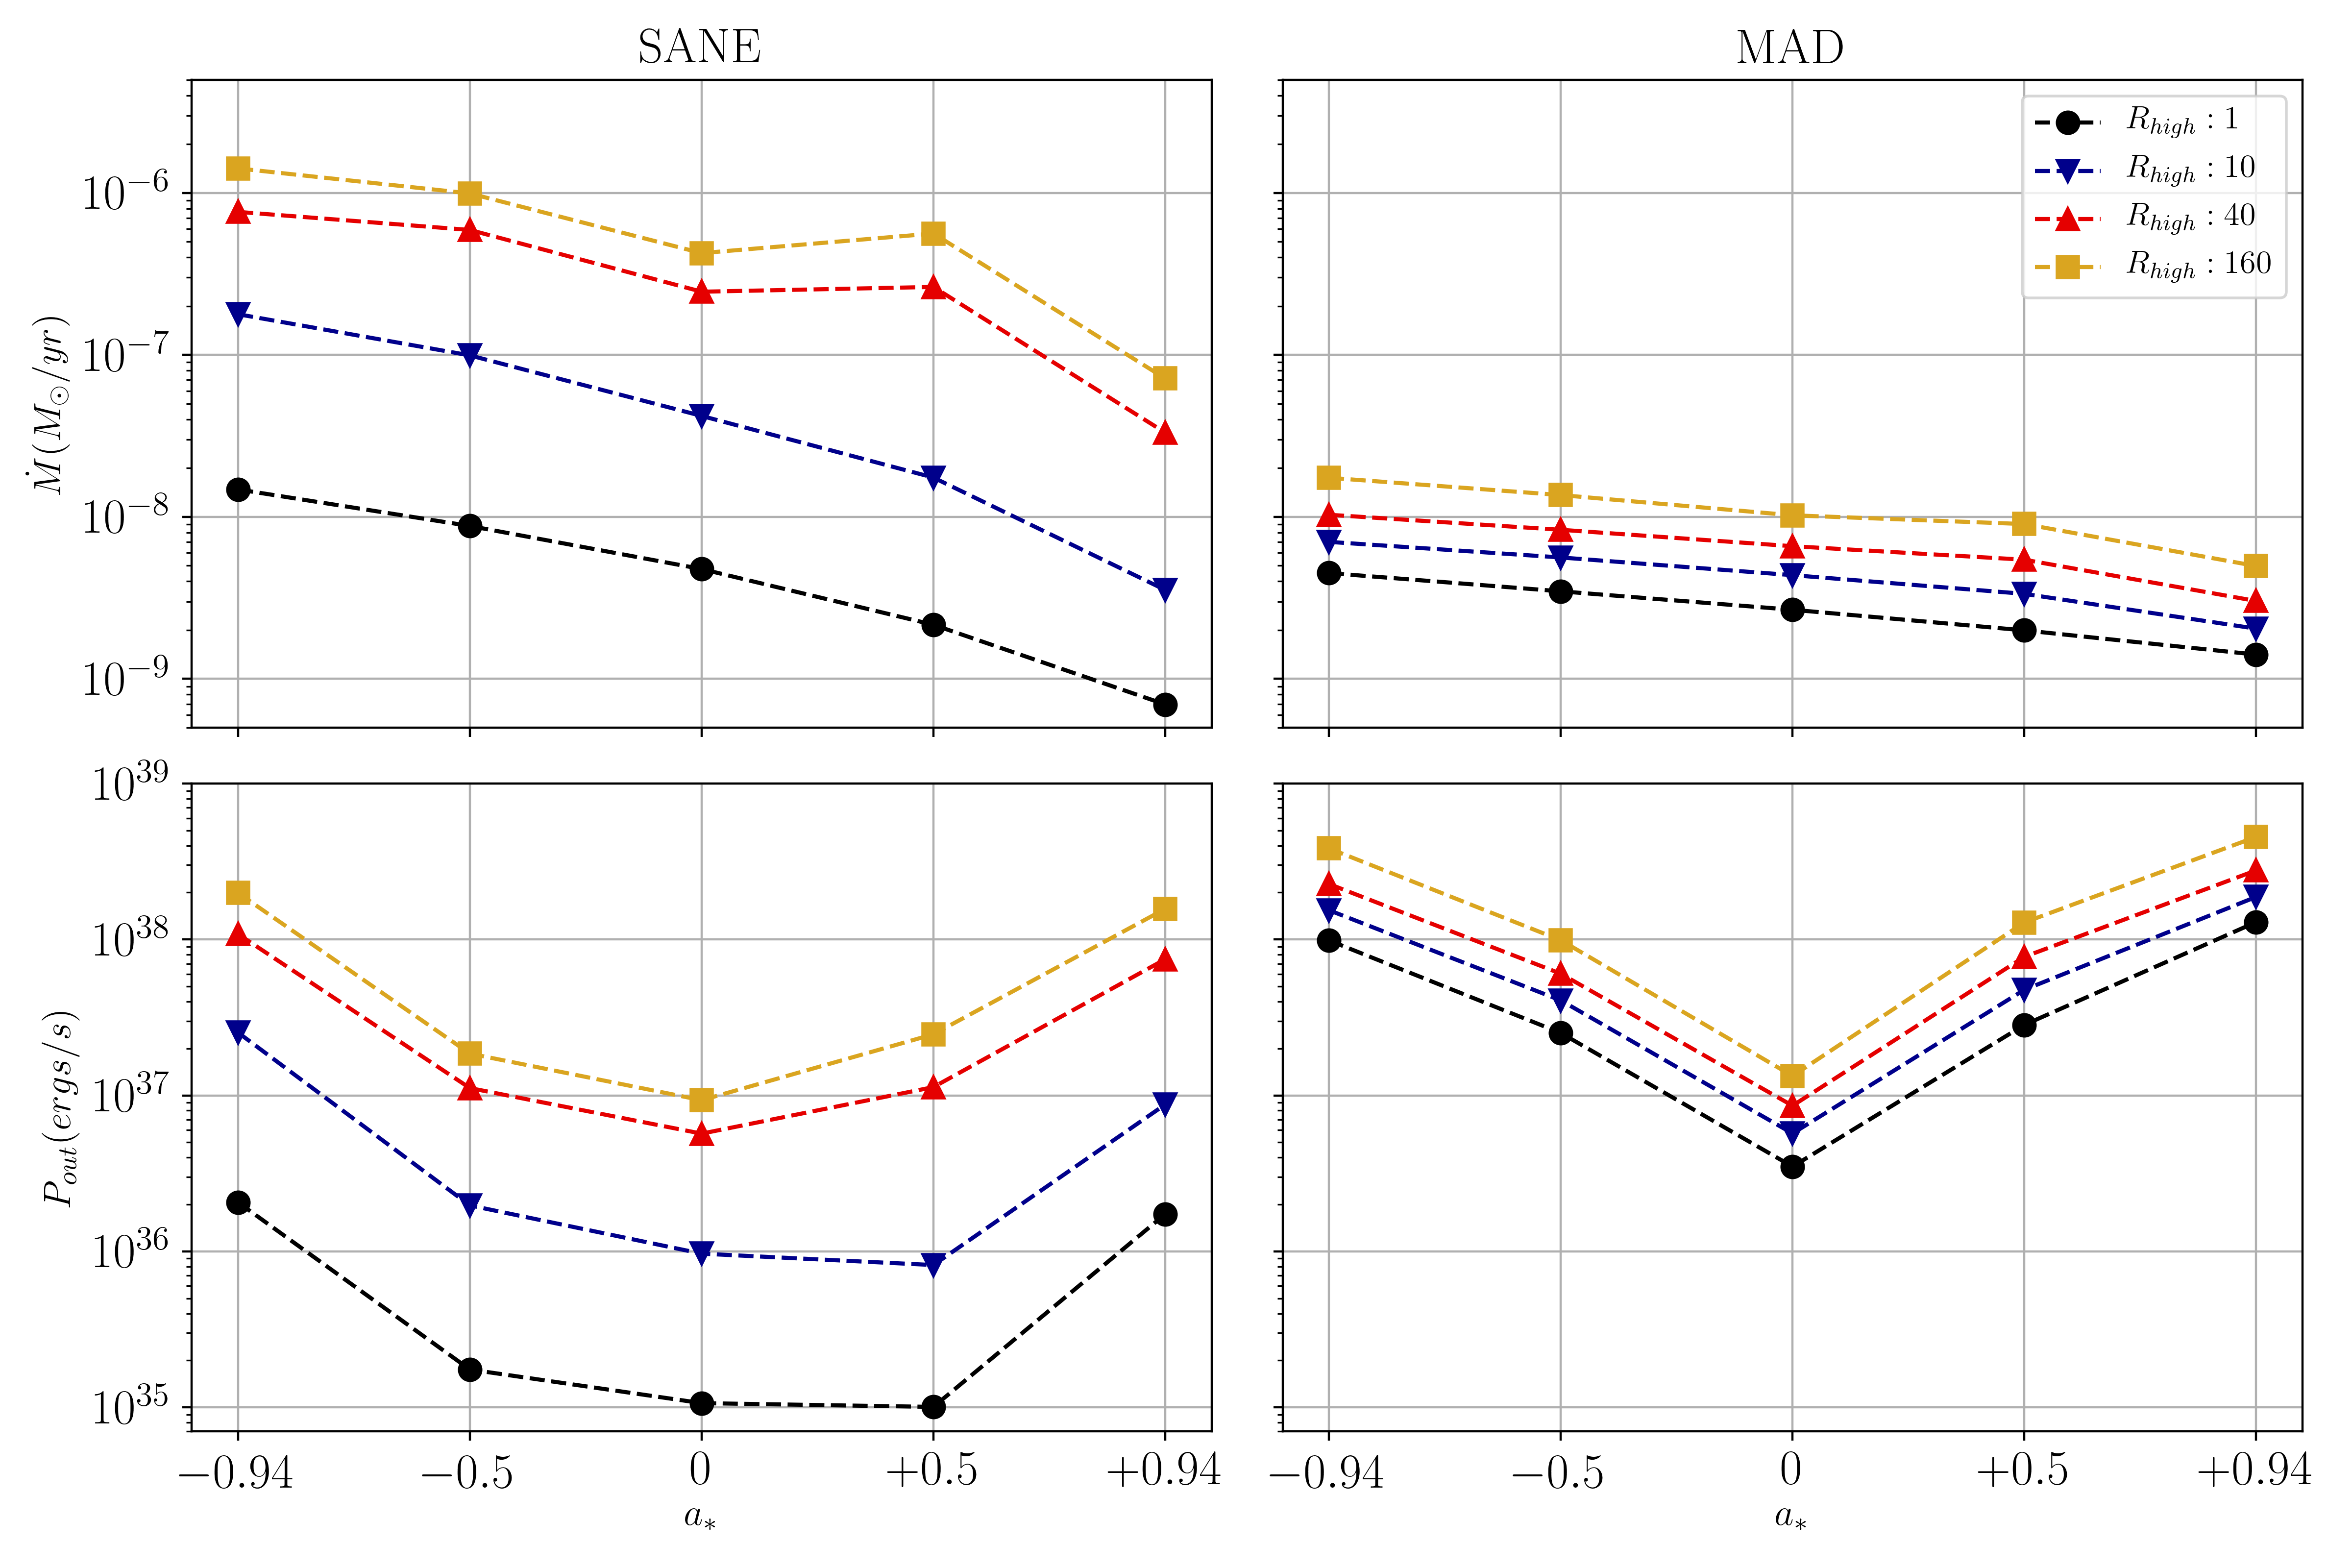
\includegraphics[width=0.95\textwidth]{figures/illinoisv3_average_mdot_pout.png}
\caption{{\it Top panels:} Accretion rates for the aligned, thermal models (\kharma data set). Since $\dot{M}$ is weakly dependent on the observer viewing angle, we plot it for a single inclination parameter, $i=50\degree$. {\it Bottom panels:} Outflow powers measured in the same models for the same observer's viewing angle. The colors and markers indicate models with different $\Rh$ parameter and they are the same in all panels.}
\label{fig:accretion_outflow_power_illinois_thermal}
\end{figure*}
% \begin{figure*}
% \centering
% 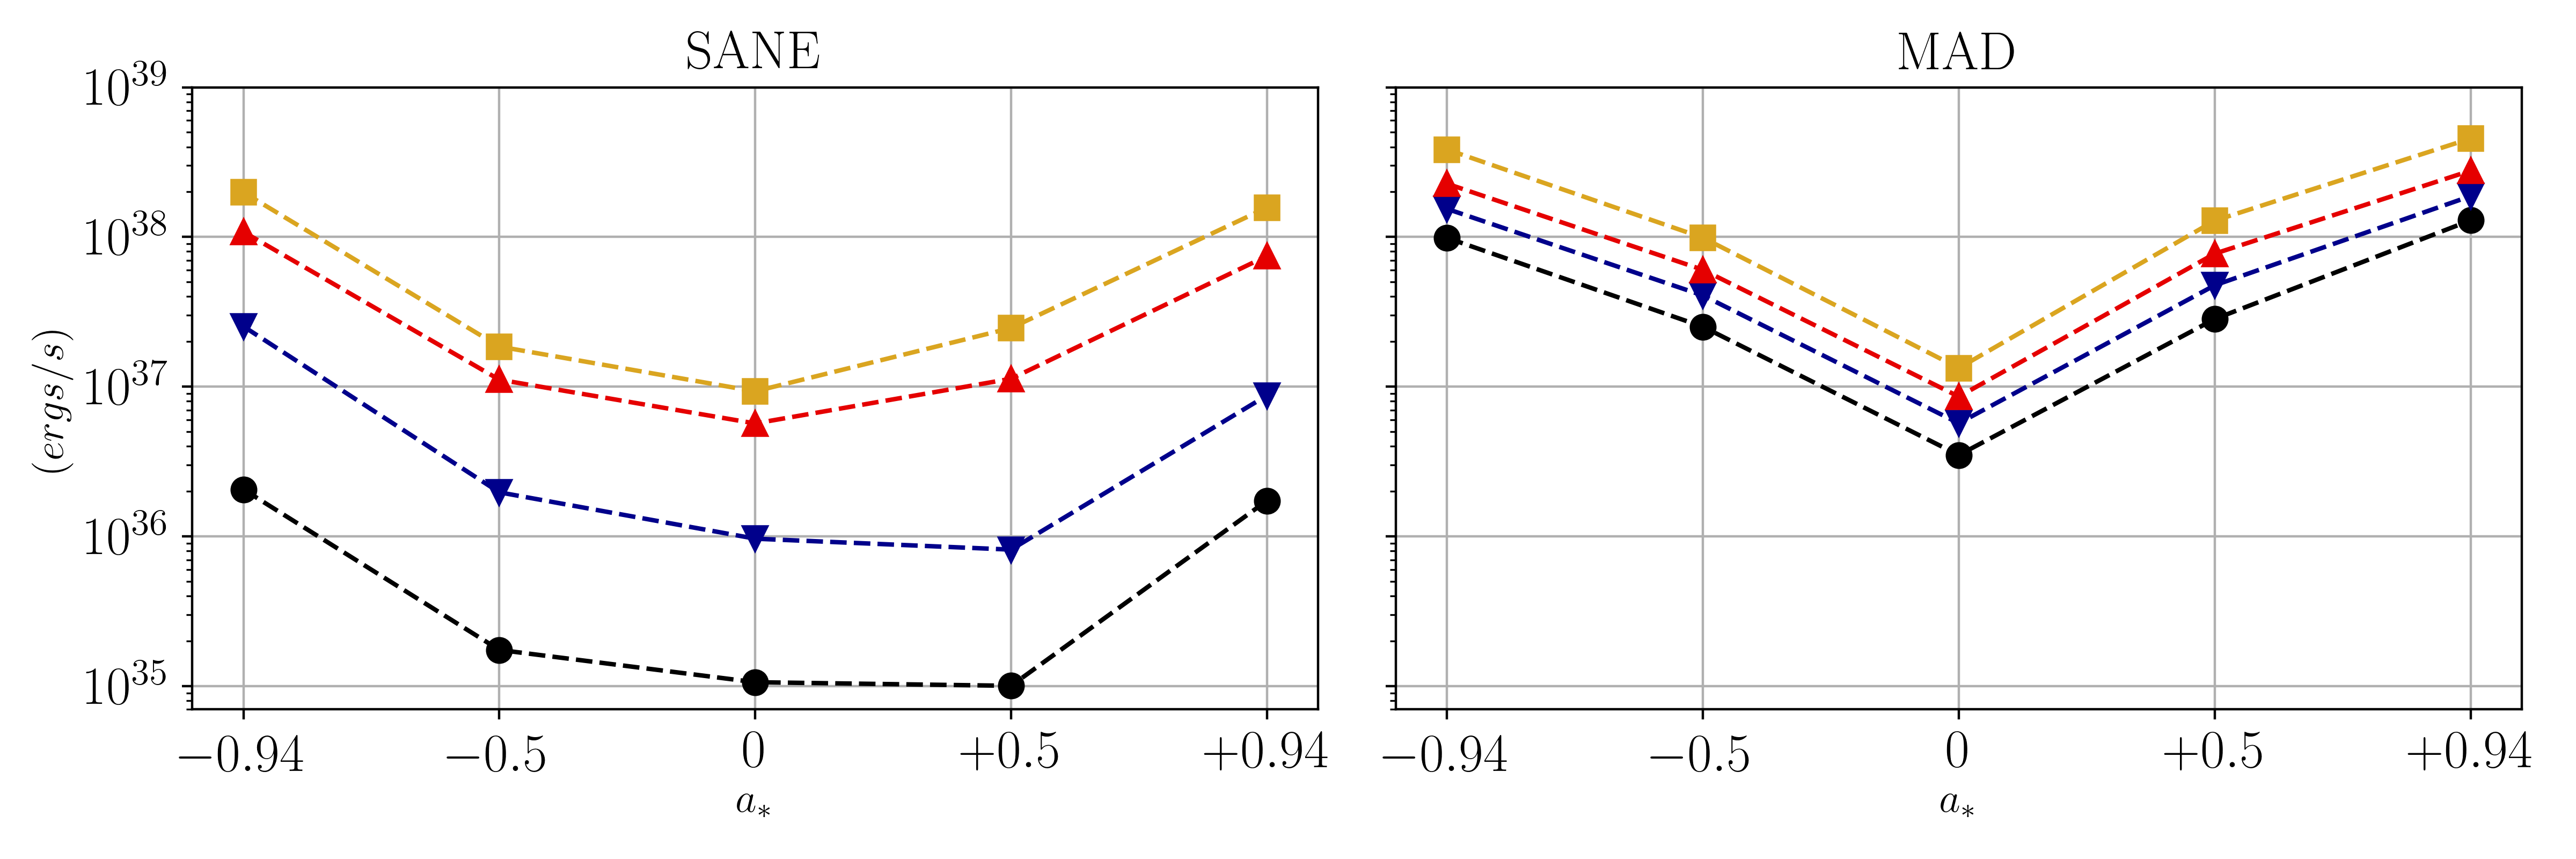
\includegraphics[width=0.95\textwidth]{figures/illinoisv3_average_outflow_power.png}
% \caption{Outflow powers measured in \kharma thermal models at an observer inclination $i=50^{\circ}$. The colors and markers are the same as \ref{fig:accretion_illinois_thermal}.}
% \label{fig:outflow_illinois_thermal}
% \end{figure*}

What is the mass accretion rate onto \sgra black hole?
%\cmf{Hector is working on the results from the BHAC runs including non-thermal emission models, should be done over the weekend}
We define the time-averaged accretion rate,
\begin{equation}
    \dot{M} = \frac{1}{\Delta t}\int dt\int d\theta d\phi\hspace{0.1cm}\sqrt{-g}\big(-\rho u^{r}\big),
\end{equation}
at the event horizon; the quantity in the parenthesis is the inward rest-mass energy flux.

In Figure~\ref{fig:accretion_outflow_power_illinois_thermal} (top panels) we show the time-averaged $\dot{M}$ (in units of solar masses per year) for the \kharma thermal models. We find the following. (i) The MAD models accrete on average, at $10^{-9}-10^{-8} M_{\odot}$yr$^{-1}$ while the SANE models have a broader range, $10^{-9}-10^{-6} M_{\odot}$yr$^{-1}$. (ii) $\dot{M}$ increases with increasing $\Rh$. Since the electron temperature inversely varies with $\Rh$, a greater $\Rh$ implies cooler electrons so to maintain an average flux density of 2.4\,Jy at 1.3\mm, the corresponding $\mathcal{M}$ increases. (iii) The SANE models exhibit a more pronounced change in $\dot{M}$ with changes in $\Rh$ as compared to the MAD models. The emission in the SANE models is predominantly from regions with large plasma $\beta$, where the electron temperature is regulated by $\Rh$; MAD models produce a significant fraction of the emission in regions with $\beta\sim 1$, where $\Rh$ does not notably influence electron temperature (cf. Figure~4 in \citetalias{M87PaperV}). (iv) The retrograde, SANE, $\Rh=40$ and $160$ models produce the largest accretion rates, $\dot{M}\sim 10^{-6}M_{\odot}$yr$^{-1}$. However, these models are ruled out due to overproduction of x-ray emission. (v) The thermal models with the critical-$\beta$ electron temperature assignment scheme predict accretion rates that lie between the $\Rh=10$ and 40 values for the chosen set of parameters ($f=0.5$, $\beta_\mathrm{crit}=1$).
\color{red}{\bf please add if bhac confirms this general trends. add figure but it would be best to plot this all together using maybe more transparent lines for bhac sims in the existing figure.}
\color{black}

Linear polarization and Faraday rotation measurements of \sgra emission at millimeter and sub-millimeter wavelengths (\citealt{2000ApJ...538L.121A, 2000ApJ...545..842Q, 2003ApJ...588..331B, 2006ApJ...640..308M, 2006JPhCS..54..354M, 2006ApJ...646L.111M}), and X-ray emission (\citealt{2003ApJ...591..891B, doi:10.1126/science.1240755}), in conjunction with semi-analytic models estimate \sgra accretion rate to be $\dot{M} \sim 10^{-9} - 10^{-7} M_{\odot}$yr$^{-1}$. The broad range of values is due to the differences in regions of radio emission in the theoretical models that are considered (ADAFs: \citealt{1998ApJ...492..554N, Yuan_2003}; Jet models: \citealt{1993A&A...278L...1F, 2000A&A...362..113F}). All our MAD model accretion rates  fall within the range of these historical observational estimates. Interestingly almost all SANE models with larger $\rhigh$ parameter (except SANE $a_*=+0.94$, which is one of our best models) have accretion rates that are inconsistent with the expectations.

\color{red}
{\bf LEFT OVER COMMENT TO INCORPORATE: Models at the highest accretion rate are ruled out by overproduction of x-ray emission.  If our models were in equilibrium over a larger range in radius, bremss from larger radius might increase the x-ray flux and disfavor more models.}
\color{black}

Our numerical simulations of black hole accretion in \sgra consistently produce relativistic outflows in the polar regions (in the standard models these outflows can be divided into disk wind/corona and relativistic jet that is often strongly magnetized and nearly hollow). These relativistic outflows have an electromagnetic energy that is typically comparable or larger than the bolometric luminosity of \sgra. We are interested in the outflow power to predict if an outflow can be observed e.g., at larger distances from the black hole where the outflow energy gets dissipated.

In the past, several authors have defined the jet outflow differently: \citet{refId0}, \citet{2014A&A...570A...7M} use a Bernoulli parameter Be, while \citealt{10.1111/j.1365-2966.2012.22002.x} consider the ratio of energy flux to rest mass flux $\mu$, and \citetalias{M87PaperV} apply a $\beta\gamma$ cut to define $P_{jet}$. Here we evaluate the total, mechanical, outflow power near the poles using \citetalias{M87PaperV}:
\begin{equation}
    P_{out} = \frac{1}{\Delta t}\int dt \int d\phi  \int_{poles}d\theta \sqrt{-g}\left(-T^{r}_{t}-\rho u^{r}\right),
\end{equation}
where $poles$ means regions where $\theta<1$ or $\theta>\pi-1$. The integral is evaluated at $r=100GM/c^{2}$ and we consider only those zones where there is outflow, i.e. the quantity in the parentheses is positive. $P_{out}$ is a broad definition for energy outflow at the polar caps that includes both the narrow, relativistic jet and the nonrelativistic winds close to the jet-disk boundary.

%In Figure~\ref{fig:outflow_illinois_thermal}
In Figure~\ref{fig:accretion_outflow_power_illinois_thermal}
(bottom panels) we show
the time-averaged, outflow power in the \kharma thermal models. As expected, the $P_{out}$ increases with increasing magnitude of black hole spin $|a_{*}|$. SANE simulations have $P_{out}$ in range $\sim 10^{35}-10^{38} \ergsps$ and $P_{out}$ is sensitive to $\rhigh$ parameter (models with larger $\rhigh$ have higher accretion rates and therefore stronger magnetic fields). For MAD models $P_{out}$ is, on average, even larger and less sensitive to $\rhigh$ and is in range of $P_{out} \sim 10^{37}$--$10^{39} \ergsps$.
\color{red}{\bf please add results from bhac for comparison if they are available.}\color{black}
\color{red}{\bf one should say a few words how electron distribution function changes mass accretion rate estimates and jet powers.}\color{black}

Many of our high spin or high $\rhigh$ models attain an outflow power $P_{out} \sim 10^{38} \ergsps$. Following \citet{2007MNRAS.379.1519M} one may ask: is it possible to hide such powerful outflow in the Galactic Center? Unlike for \m87, there is no observational estimate for power of a putative jet in \sgra system. There have been several studies at radio, X-ray and $\gamma$-ray that have suggested the presence of a mildly relativistic outflow based on morphological structures observed in the \sgra complex (\citealt{2012ApJ...758L..11Y,2012AAS...22051303S,Li_2013,2019ApJ...875...44Z,2021arXiv210713402B} and references therein). However, due to the low luminosity of \sgra and the presence of the interstellar scattering screen (\citealt{2016ApJ...824...40O,2017MNRAS.471.3563D,2018ApJ...865..104J,2019A&A...621A.119B}) there is no direct evidence of the jet or outflow from \sgra. \monika{EHT data interpretation suggest that we cannot exclude the presence of an outflow.???}


%==============================================================================
\subsection{Caveats and Limitations}\label{sec:limits}


%%%%%%%%%%%%%%%%%%%%%%%%%%%%%%%%%%
% \note{to be discussed: how much we would like to discuss polarization emission?}\textcolor{red}{RJA: We should mention the M87 Polarization Collaboration papers \cite{M87PaperVII}, including a comparison of whether Sgr A* is similar enough (e.g., MAD with vertical fields Faraday depolarized on much of the accretion flow) to have an azimuthally spiral EVPA pattern. Figures in  \citep{Emami2021} have similar morphology}.

% \hyp{to-do :  adding historical RIAF fitting result to proto-EHT observations; how recent  GRMHD simulation and subsequent GRRT post-processing suggest other key parameters onto the Broderick 2005 RIAF model; jet componenet? cross referencing MCFE RIAF analysis product?} A proto-EHT array described in \cite{Doeleman2008} estimated the Sgr A* emitting region profile as a circular Gaussian with intrinsic size $37^{+16}_{-10}\ \mu$as.

% % EHT flux vs. baseline observations constrain the emitting region intrinsic size to 37 microarcseconds for a circular Gaussian emission profile

% More recent measurements of closure phases of a few degrees \cite{Fish2016} suggest an asymmetric ring-like profile, with major axis 56 microarcseconds
%%%%%%%%%%%%%%%%%%%%%%%%%%%%%%%%%%

%------------------------------------------------------------------------------
\subsubsection{Collisionless plasma effects}

\monika{some of the collisionless aspects are addressed in appendix C1 in subsection on selfconsistent electron heating models. check if this is mentioned below}
\br{I rewrote a little bit and added a sentence.}

{The mean free path to collisions for particles is typically larger than or comparable to the system size for the accretion disk of \sgra, rendering its plasma collisionless. The GRMHD models employed in this work, describe a collisional system, whereas a first-principles modeling of the collisionless plasma requires a fully kinetic treatment. General relativistic (radiative) kinetic simulations are crucial for dynamically probing the electron temperature, effects of non-thermal distribution functions, and pressure anisotropy and their interplay with radiation in collisionless plasma in the accretion disk and jet. While global general relativistic kinetic simulations cannot be performed with full physical separation between microscopic plasma scales (the particle's Larmor radius $r_{\rm L}$, and plasma skin depth $d_{\rm e}$) and macroscopic scales (the gravitational radius $r_{\rm g}$), they can achieve the right hierarchy of scales ($r_{\rm g} \gg d_{\rm e} \gg r_{\rm L}$) for magnetized plasmas \citep{2018A&A...616A.184L,2018ApJ...863L..31C,2019PhRvL.122c5101P,2020PhRvL.124n5101C,2020ApJ...895..121C,2020ApJ...902...80K,2021A&A...650A.163C,2021PhRvL.127e5101B}. Even in GRMHD, it is computationally challenging to resolve plasma heating processes powering the observed radiation in a converged manner. It is currently not yet feasible to resolve dissipation at the smallest scales of the turbulent cascade or the interplay between turbulence and reconnection at a similar level as in local box simulations \citep{2012ApJ...755...50R,2013ApJ...773..118H,2015PhRvL.114f1101H,2016PhRvL.117w5101K,2017PhRvL.118e5103Z,2018PhRvL.121y5101C,2018ApJ...859..149I,2019PhRvL.122e5101Z,2021ApJ...921...87N,2021arXiv211108188C}. However, \citet{2019ApJS..243...26P} and \citet[in prep.]{Olivares_et_al} show that the global accretion dynamics (mass accretion rate, magnetic flux on the horizon, and MRI quality factor) are converging between the different simulations in this work. Kinetic processes in the (near-)collisionless plasma may increase the effective particle collision rate \citep[see e.g.,][]{2016PhRvL.117w5101K}. Deviations from the infinitely conductive ideal fluid approximation may alter the thermodynamics of the flow \citep[see e.g., ][and Appendix C1]{2017MNRAS.470.2240F}. Some aspects of (near-)collisionless plasma dynamics can be described with non-ideal effects (e.g., viscosity, resistivity, heat conduction, pressure anisotropy) in GRMHD models for black hole accretion, e.g.,  \cite{2014MNRAS.440L..41B,2015ApJ...810..162C,2016MNRAS.456.1332F,2017ApJ...837...92C,2017MNRAS.470.2240F,2018ApJ...859...28Q,2019ApJS..244...10R,2019ApJ...882....2V,2020ApJ...900..100R,2021PhRvD.104j3028M,2021arXiv211103689N,2021arXiv211105752M}. For example, the first efforts have recently been made with high-resolution global GRMHD simulations to capture heating through magnetic reconnection in the largest current sheets in the system \citep{2020MNRAS.495.1549N,2020ApJ...900..100R,2021MNRAS.508.1241C,2021arXiv210915115R,2021arXiv211103689N}.}

%------------------------------------------------------------------------------
\subsubsection{Positrons}\label{sec:pair}

\monika{i think this section should start with some general statement why do we want to consider positrons at all.}
\ckc{I refer to this section from the eDF section.  Please feel free to move this around as long as we keep the label.}

\monika{Also, is it possible to incorporate this positron story into Caveats and Limitations?}
\br{I would add it as a subsection (with a subtitle) of the caveats, and it indeed needs a general statement why we want to consider positrons (I would mention magnetosphere (or potential jet that we dont see?) is pair plasma, and (non-thermal) positrons (accelerated in a gap, or by a current sheet in the jet/magnetosphere) can be mixed into the disk through reconnection or instabilities at the jet base, injecting non-thermal magnetized blobs into the disk}\monika{arent most of the collisionless kinetic plasma simulations you report above actually done for electron-positron plasmas? i think this should be maybe connected somehow}\br{I would not mix those paragraphs but do it as you did now (with separate subtitles), because the main point the two paragraphs are making is different (I think the current subtitles reflect that well). We could indeed connect an introducing sentence of this positron paragraph to the collisionless paragraph:}


\br{``The black hole magnetosphere or potential jet region may consist mainly of highly magnetized electron-positron pair plasma produced by pair discharges. The pair plasma can be accelerated to non-thermal power-law energy distributions in spark gaps or reconnecting current sheets \citep{2018A&A...616A.184L,2018ApJ...863L..31C,2019PhRvL.122c5101P,2020PhRvL.124n5101C,2020ApJ...895..121C,2020ApJ...902...80K,2021PhRvL.127e5101B} and potentially get mixed into the accretion disk through the exhaust of the reconnection layer \citep{2021arXiv210915115R}.''}


\cite{2006MNRAS.367..905B} devised a canonical model of Sgr A* as a  radiatively inefficient accretion flow (RIAF). Semi-analytic RIAF models implementing  this using the general relativistic ray tracer GRTRANS \citep{2016MNRAS.462..115D} can be found in  \cite{2021arXiv210105327E}, where  positrons are included using emission modeling motivated in  \cite{2020ApJ...896...30A}. The Figs. 1-3 %\ref{fig:EmamiRIAF}
models from \cite{2021arXiv210105327E} shows Stokes maps and polarized spectra of a \cite{2006MNRAS.367..905B} RIAF with plasma $\beta=10$ and 1$\%$ of the emitting particles nonthermal electrons. The near-extremal ($a/M=0.998$) model shown exhibits Doppler boosting asymmetry in a crescent-shaped intensity pattern with a spiral global electric vector polarization angle (EVPA) pattern and polarization preferentially distributed within this region.

\hyp{As phenomenological models are not considered in this work, the position effect in this subsection may rewrite in a way only focus on the resulting effects and its possible impact for the model images. That is, we may consider to skip the previous paragraph.}
The addition of small non-thermal populations of positrons \citep{2020ApJ...896...30A,2021arXiv210105327E} tends to: increase overall intensity in jet regions for fixed electron number density; modify the low-frequency spectral slope; cancel the observed intrinsic circular polarization and enhance circular polarization due to Faraday conversion. The last of these positron effects is particularly apparent when comparing declining tails of x-ray spectra of positron-rich versus positron-poor sources, as seen in \cite{2021arXiv210105327E}.%Fig. \ref{fig:EmamiRIAFSpectra}.

However, positron effects for Sgr A* are severely limited by the compactness \citep{2012MNRAS.424L..26G} due to the low observed luminosity and outflow geometry. In fact \cite{2011ApJ...735....9M} estimate the funnel positron pair density of Sgr A* to be $10^{-8}\mathrm{cm}^{-3}$ (well below the Goldreich-Julian density required to screen plasma electric fields). By contrast, the comparable density for M87 is $10^3\mathrm{cm}^{-3}$.



%MOVED from Sect. 3.1 to Sect. 3.0
% \textcolor{red}{RJA: Include a summary of analytic/semi-analytic models and Sgr A* simulations in the Literature} Analytic disk $\alpha$-model for angular momentum transport \cite{Shakura1973}. Semi-analytic model motivated in \cite{Yuan2003} and expanded in \cite{Broderick2011}. GRMHD Simulation with hotspots reproducing Sgr A* flares \cite{Ripperda2020}.

%==============================================================================
\subsection{Future Constraints}\label{sec:future}

\begin{itemize}

\item SANE/MAD will be settled by polarization, but that is beyond the scope of this paper

\item Shows value of contemporaneous GMVA observations

\item We cannot assess the sense of rotation.
Future analysis can potentially extract sense of rotation.  Sensitive to inclination: the edge-on models "flash" simultaneously over all PAs, while face-on exhibits rotation.

\item note on fitting riafs?

\item do we need better models or better data in the future to e.g. measure the spin of the black hole in \sgra?

\end{itemize}

